\textbf{LeVeque 3.2} 

a) Show that the 9-point Laplacian (3.17) has the truncation error derived in Section 3.5. \textbf{Hint: } To simplify
   the computation, note that the 9-point Laplacian can be written as the 5-point Laplacian (with known truncation 
   error) plus a finite difference approximation that models $\frac{1}{6} h^2 u_{xxyy} + \mathcal{O}(h^4)$.

\begin{solution}\ \\\\
   Let $\nabla_5^2 \bar{u}$ denote the 5-point stencil for the Laplacian of $\bar{u} = u_{i,j}= u(x_i, y_j) $, given by:
   
   \begin{align*}
      \nabla_5^2 \bar{u} = \frac{1}{h^2} (u_{i-1, j} + u_{i+1, j} + u_{i, j-1} + u_{i, j+1} - 4\bar{u})
   \end{align*}

   Then the 9-point stencil for the Laplacian of $u$ at $(x_i, y_j)$ may be written in terms of the 5-point stencil:

   \begin{equation}
      \nabla_9^2 \bar{u} = \frac{1}{6h^2} [4h^2 \nabla_5^2 \bar{u} + (u_{i-1, j-1} + u_{i-1, j+1} + u_{i+1, j-1} + u_{i+1, j+1}) - 4\bar{u}]
   \end{equation}

   Since the truncation error for the 5-point Laplacian is known to be\footnote{
      See Section 3.4 p. 63 of LeVeque
   } \linebreak
   $\frac{1}{12} h^2 (\bar{u}_{xxxx} + \bar{u}_{yyyy}) + \mathcal{O}(h^4)$, we have:

   $$
      \nabla_5^2 \bar{u} - \nabla^2 \bar{u} = \frac{1}{12} h^2 (\bar{u}_{xxxx} + \bar{u}_{yyyy}) + \mathcal{O}(h^4) \\
   $$

   and hence:

   \begin{equation}
      \nabla_5^2 \bar{u} = \frac{1}{12} h^2 (\bar{u}_{xxxx} + \bar{u}_{yyyy}) + \nabla^2 \bar{u}  + \mathcal{O}(h^4).
   \end{equation}

   With this result in our back pockets, we turn our attention to the \linebreak
   $u_{i-1, j-1} + u_{i-1, j+1} + u_{i+1, j-1} + u_{i+1, j+1}$ term, which we analyze by way of multivariate Taylor 
   series expansion of $u(x_i + \Delta x, y_j + \Delta y)$ about $\bar{u} = u(x_i, y_j)$. We explicitly write out the
   fourth-order expansion:

   \begin{alignat*}{2}
      u(x_i + \Delta x, y_j + \Delta y) &= \sum\limits_{|\alpha| \le 4}{\frac{D^{\alpha}\bar{u}}{\alpha!} (\Delta x, \Delta y)^\alpha} + \mathcal{O}(h^5) \\
                                        &= \bar{u} + \bar{u}_{x} \Delta x + \bar{u}_{y} \Delta y \\
                                        &+ \frac{1}{2!} \bar{u}_{xx}(\Delta x)^2 + \bar{u}_{xy} \Delta x \Delta y + \frac{1}{2!} \bar{u}_{yy}(\Delta y)^2 \\
                                        &+ \frac{1}{3!} \bar{u}_{xxx}(\Delta x)^3 + \frac{1}{2!} \bar{u}_{xxy} (\Delta x)^2 \Delta y + \frac{1}{2!} \bar{u}_{xyy} \Delta x (\Delta y)^2 + \frac{1}{3!} \bar{u}_{yyy}(\Delta y)^3 \\
                                        &+ \frac{1}{4!} \bar{u}_{xxxx}(\Delta x)^4 + \frac{1}{3!} \bar{u}_{xxxy} (\Delta x)^3 \Delta y + \frac{1}{2! 2!} \bar{u}_{xxyy} (\Delta x)^2 (\Delta y)^2  \\
                                        &+ \frac{1}{3!} \bar{u}_{xyyy} \Delta x (\Delta y)^3 + \frac{1}{4!} \bar{u}_{yyyy}(\Delta y)^4 + \mathcal{O}(h^5).
   \end{alignat*}

   In particular, we note that for e.g., $u_{i-1, j+1} = u(x_i - h, y_j + h)$, we have that $\Delta x = -h$ and hence
   any term with an odd power of $\Delta x$ is negative with respect to the rest of the term. By symmetry, every such 
   term cancels with a corresponding term when summed with $u_{i+1, j+1}$. Moreover, when we sum 
   $u_{i-1, j-1} + u_{i-1, j+1} + u_{i+1, j-1} + u_{i+1, j+1}$, all terms with an odd power of $\Delta y$ cancel\footnote{
      In the case that both powers of $\Delta x$ and $\Delta y$ are odd, such terms in $(u_{i-1, j-1} + u_{i+1, j+1})$
      cancel with corresponding terms in $(u_{i-1, j+1} + u_{i+1, j-1})$.
   }, and so we are left only with terms in the above expression which contain even powers of both $\Delta x$ and 
   $\Delta y$.  Furthermore, all fifth-order terms must contain odd powers of either $\Delta x$ or $\Delta y$ (just as
   with the third-order terms above), and so the sum 
   $u_{i-1, j-1} + u_{i-1, j+1} + u_{i+1, j-1} + u_{i+1, j+1}$ becomes the following sixth-order expansion:

   \begin{align*}
      u_{i-1, j-1} + u_{i-1, j+1} + u_{i+1, j-1} + u_{i+1, j+1} &= 4 \bar{u} + \frac{4}{2!} \bar{u}_{xx}(\Delta x)^2 + \frac{4}{2!} \bar{u}_{yy}(\Delta y)^2 \\
                                        &+ \frac{4}{4!} \bar{u}_{xxxx}(\Delta x)^4 + \frac{4}{2! 2!} \bar{u}_{xxyy} (\Delta x)^2 (\Delta y)^2  \\
                                        &+ \frac{4}{4!} \bar{u}_{yyyy}(\Delta y)^4 + 4 \mathcal{O}(h^6).
   \end{align*}

   In the case that $\Delta x = \Delta y = h$, the above equation reduces to:

   \begin{align*}
      u_{i-1, j-1} + u_{i-1, j+1} + u_{i+1, j-1} + u_{i+1, j+1} &= 4 \bar{u} + 2 h^2 \nabla^2 \bar{u}
                                                                   + h^4 \left(\frac{1}{6}\bar{u}_{xxxx} + \bar{u}_{xxyy} +  \frac{1}{6}\bar{u}_{yyyy}\right) + \mathcal{O}(h^6).
   \end{align*}

   \pagebreak
   Substituting this result along with (2) into (1) yields the following expression for the 9-point Laplacian:

   \begin{align*}
      \nabla_9^2 \bar{u} &= \frac{1}{6h^2} \left[
                           \frac{1}{3} h^4 (\bar{u}_{xxxx} + \bar{u}_{yyyy}) + 6 h^2 \nabla^2 \bar{u}
                              + h^4 \left(\frac{1}{6}\bar{u}_{xxxx} + \bar{u}_{xxyy} + \frac{1}{6}\bar{u}_{yyyy}\right) + \mathcal{O}(h^6)
                           \right] \\
                         &= \frac{1}{6h^2} \left[
                              6 h^2 \nabla^2 \bar{u} 
                              + \frac{1}{2} h^4 \left(\bar{u}_{xxxx} + 2 \bar{u}_{xxyy} + \bar{u}_{yyyy}\right) 
                              + \mathcal{O}(h^6)
                           \right] \\
                         &= \nabla^2 \bar{u} + \frac{1}{12} h^2 \nabla^2(\nabla^2 \bar{u}) + \mathcal{O}(h^4) \\
                         &= \nabla^2 \bar{u} + \frac{1}{12} h^2 \nabla^2 f(x_i, y_j) + \mathcal{O}(h^4).
   \end{align*}

   Hence our (local) truncation error at $(x_i, y_j)$is given by:
   
   $$
      \tau_{ij} = \nabla_9^2 \bar{u} - \nabla^2 \bar{u} = \frac{1}{12} h^2 \nabla^2 f(x_i, y_j) + \mathcal{O}(h^4).
   $$

   as desired.
   \ \\\\
\end{solution}

\pagebreak
b) Modify the \texttt{MATLAB} script \texttt{poisson.m} to use the 9-point Laplacian (3.17) instead of the 5-point
   Laplacian, and to solve the linear system (3.18) where $f_{ij}$ is given by (3.19). Perform a grid refinement study
   to verify that fourth order accuracy is achieved.

\begin{solution}\ \\\\
    Our computed relative error for $\Omega = [0, 1] \times [0, 1]$ with decreasing grid size is shown below:

    \begin{figure}[h]
        \begin{lstlisting}
         Computed solution on domain [0.00, 1.00] x [0.00, 1.00]:

         Grid points      Grid size (hx, hy)      Relative error
         -------------------------------------------------------
         ( 10,  10)       (0.100000, 0.100000)    1.161e-07
         ( 20,  20)       (0.050000, 0.050000)    7.298e-09
         ( 40,  40)       (0.025000, 0.025000)    4.571e-10
         ( 60,  60)       (0.016667, 0.016667)    9.031e-11
         (100, 100)       (0.010000, 0.010000)    1.200e-11
         
         Least squares fit gives E(h) = 0.00112631 * h^3.98833
        \end{lstlisting}
        \caption{Output of \texttt{problem\_2b.m} showing decreasing error resulting from grid refinement}
    \end{figure}
    
    Since our least squares fit for error is given by $E(h) = 0.00112631 h^{3.98833}$, we see that the error is 
    $\mathcal{O}(h^4)$, as expected.
    
    \begin{figure}[h]
        \centering
        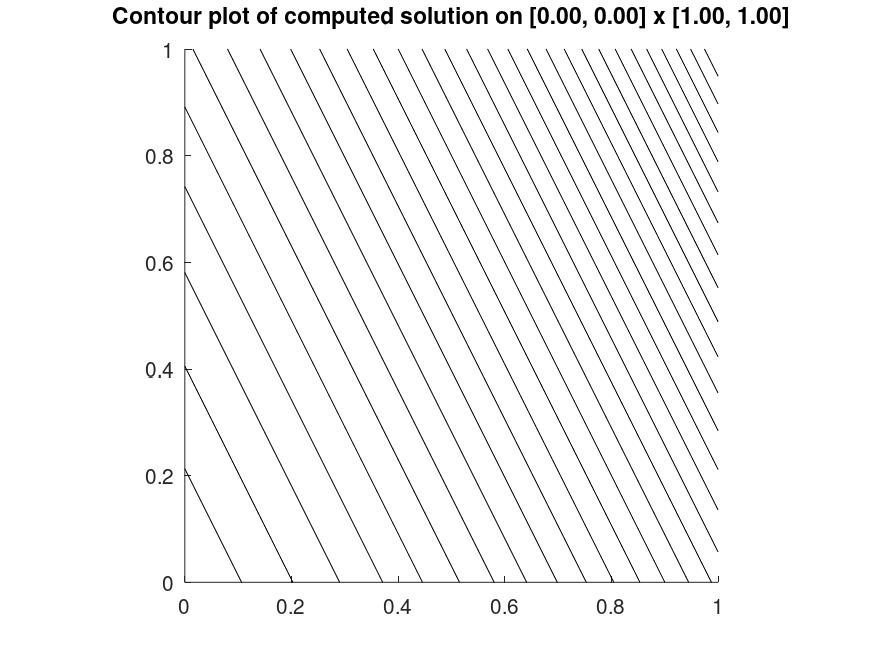
\includegraphics[width=0.6\textwidth]{poisson_9pt_stencil_0-0_1-1_hx-0.010_hy-0.010.png}
        \caption{Contour plot of solution on $[0, 1] \times [0, 1]$ with grid size $\Delta x =\Delta y = 0.01$}
    \end{figure}
\end{solution}